\documentclass[aspectratio=169]{beamer}
\setbeamertemplate{navigation symbols}{}
\usepackage{color,amsmath,comment, subfigure}
\usepackage{booktabs}
\def\vf{\vfill}
\usepackage{url}

\def\imagetop#1{\vtop{\null\hbox{#1}}} %http://tex.stackexchange.com/questions/23521/tabular-vertical-alignment-to-top

%\setbeameroption{show notes}

%%%%%%%%%%%%%%%%%%%%%%%%%%
\title[]{Class 18: Social media and individuals}
\author[]{Matthew J. Salganik}
\institute[]{Sociology 204: Social Networks\\Princeton University}
\date[]{
1/3 Overview
\vfill

\begin{flushleft}
\vspace{0.6in}

\includegraphics[width=0.1\textwidth]{figures/cc.png}
\end{flushleft}
}

\begin{document}
%%%%%%%%%%%%%%%%%%%%%%%%%%%
\frame{\titlepage}
%%%%%%%%%%%%%%%%%%%%%%%%%%%
\begin{frame}

Social media:
\begin{itemize}
\item Lecture 18: Social media and individuals \pause
\item Lecture 19: Social media and society \pause
\item Lecture 20: Social ads in social media \pause
\item Lecture 21: Fixing social media 
\end{itemize}

\end{frame}
%%%%%%%%%%%%%%%%%%%%%
\begin{frame}

\begin{center}
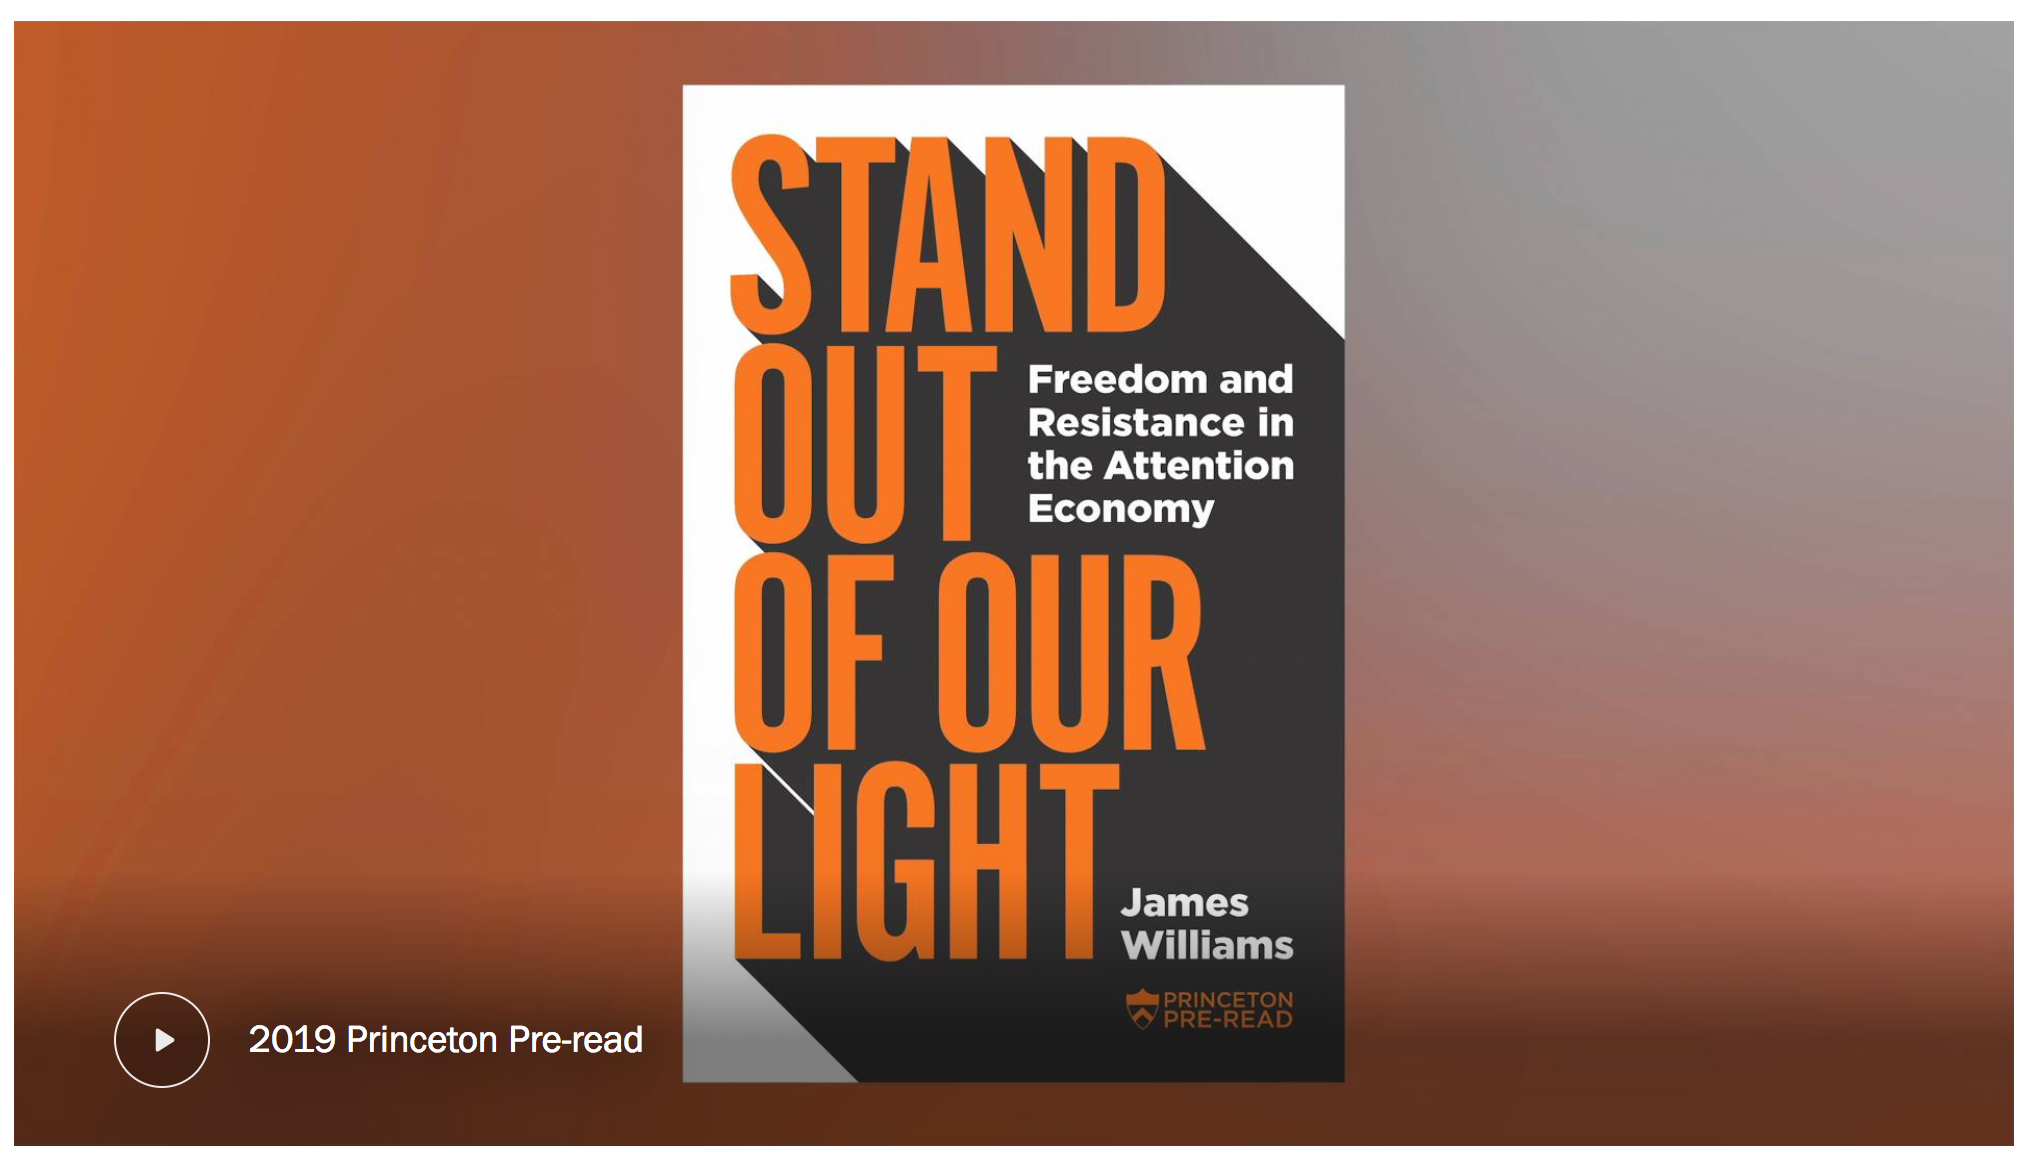
\includegraphics[width=0.9\textwidth]{figures/stand_out_of_our_light}
\end{center}
\tiny{\url{https://www.princeton.edu/news/2019/04/11/liberation-attention-digital-distraction-princeton-pre-read}}\\

\vfill
Big, important, and hard to study

\end{frame}
%%%%%%%%%%%%%%%%%%%%%
\begin{frame}

\begin{center}
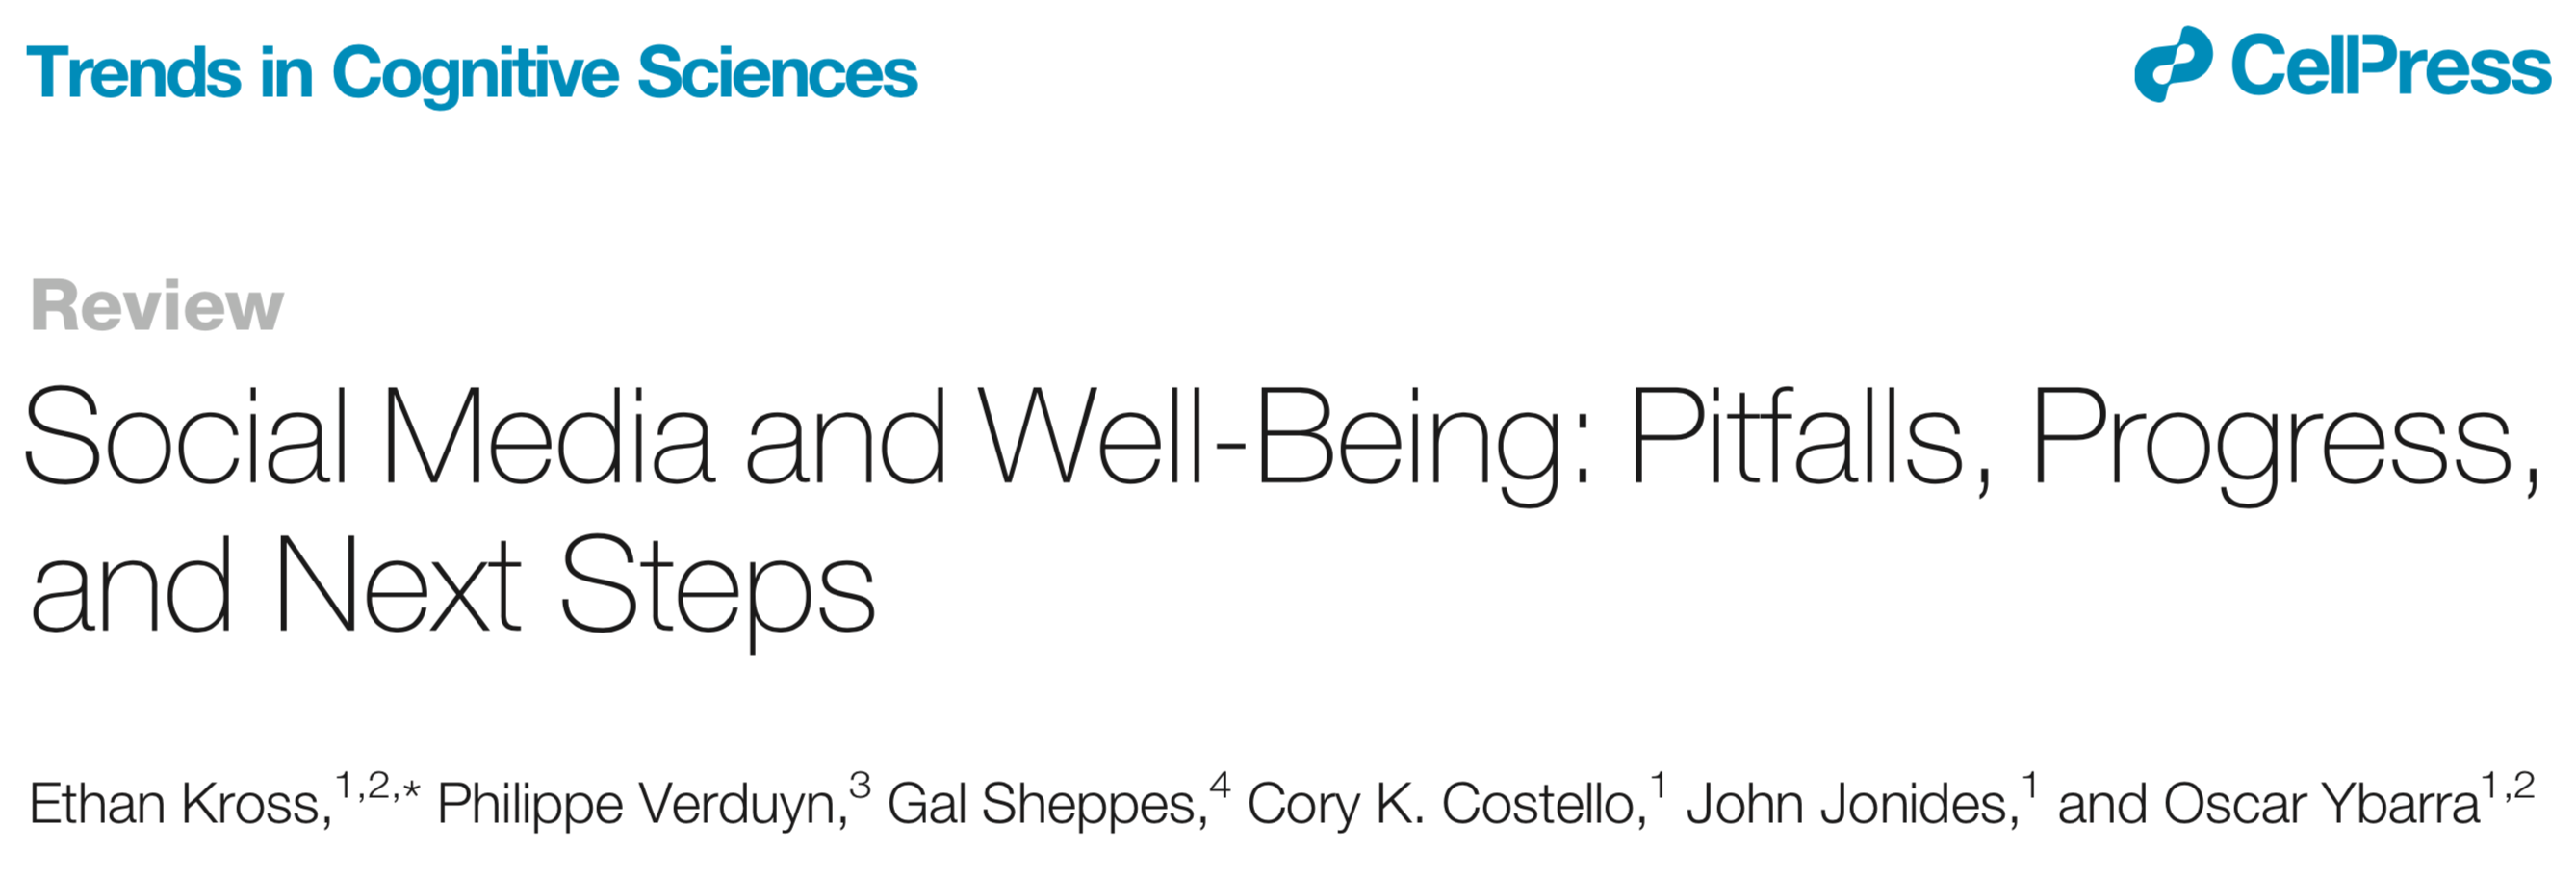
\includegraphics[width=0.8\textwidth]{figures/kross_social_2021_title}
\end{center}

\end{frame}
%%%%%%%%%%%%%%%%%%%%%%
\begin{frame}

Social media: ``online platforms that allow people to create and share information with others'' (Kross et al.\ 2021)\pause

\begin{center}
\only<2>{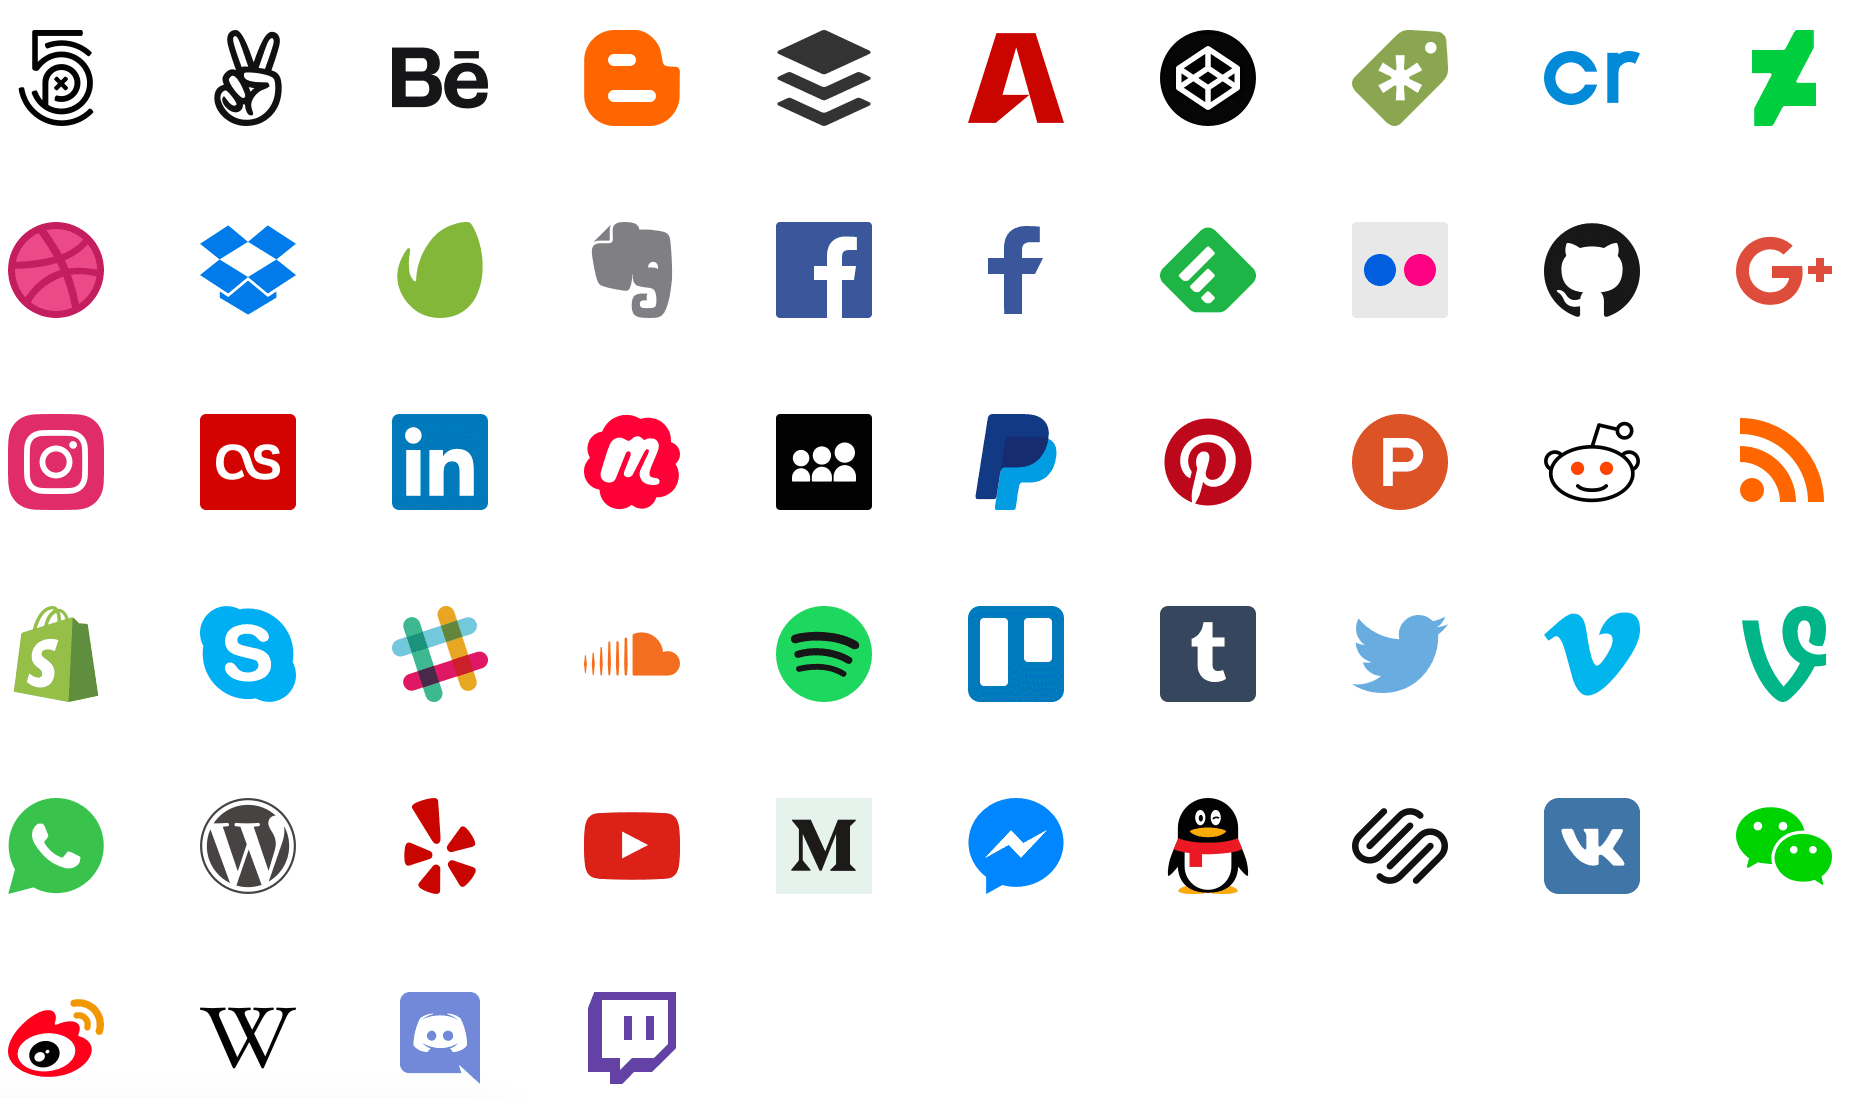
\includegraphics[width=0.8\textwidth]{figures/social_media_logos}}
\only<3->{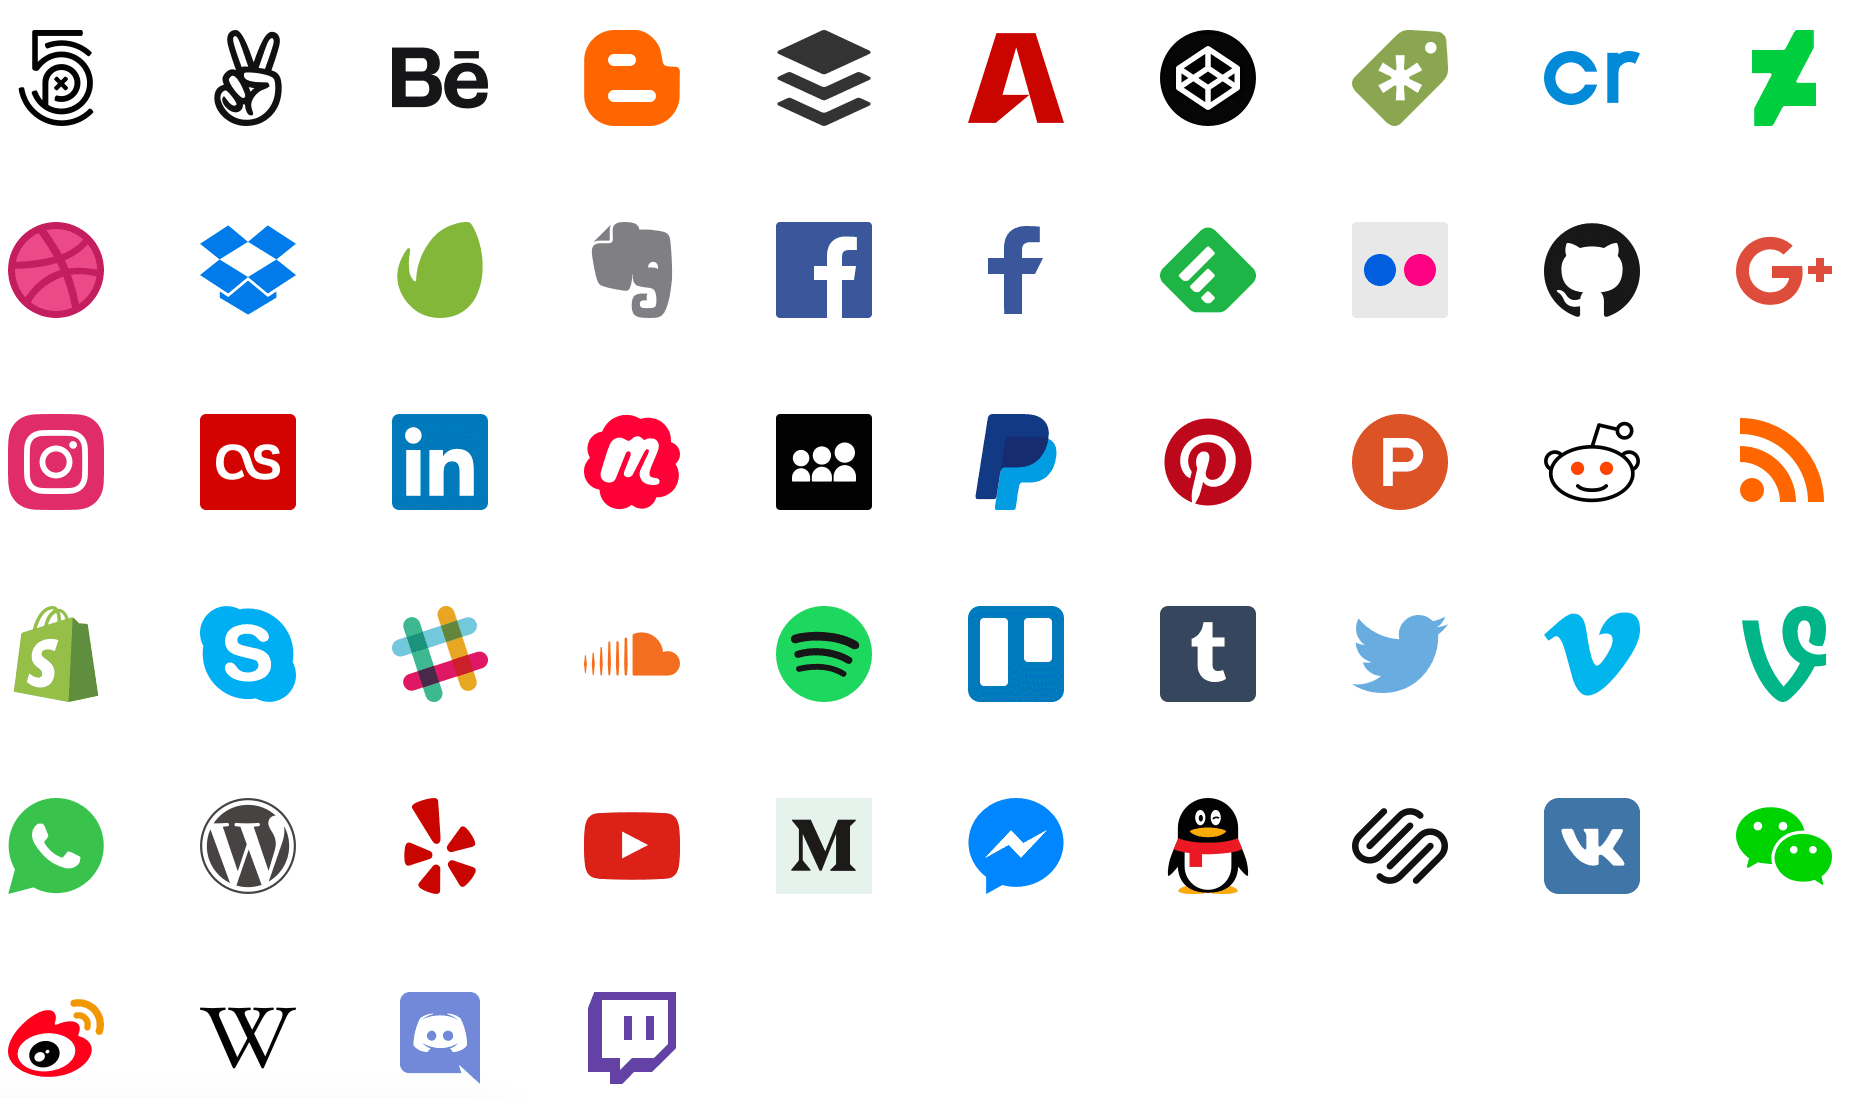
\includegraphics[width=0.3\textwidth]{figures/social_media_logos}}
\end{center}
{\tiny \url{https://nucleoapp.com/icons/social-media}}

\begin{itemize}
\item Should email be included?  What about something like Slack? \pause
\item This category called ``social media'' includes lots of quite different things. Kross et al. say this leads to ``jingle-jangle'' problem.
\end{itemize}

\end{frame}
%%%%%%%%%%%%%%%%%%%%%
\begin{frame}

Does the amount of time that people spend on social media impact their wellbeing?  First generation: cross-sectional evidence. 
\begin{itemize}
\item Inconsistent results.  Some find positive, some find negative.  
\item Perhaps differences are attributed to different platforms or different groups of people? \pause
\item Questions about what is the cause and what is the effect.\pause
\item Questions about unmeasured confounders (e.g., unemployment) \pause
\end{itemize}

\end{frame}
%%%%%%%%%%%%%%%%%%%%%
\begin{frame}

Does the amount of time that people spend on social media impact their wellbeing?  Second generation: longitudinal design, experience sampling \pause
\begin{itemize}
\item Inconsistent results.  \pause
\item Perhaps because of different operationalizations and poor accuracy of self-reported social media usage
\end{itemize}

\end{frame}
%%%%%%%%%%%%%%%%%%%%%
\begin{frame}

Does the amount of time that people spend on social media impact their wellbeing?  Third generation: experimental
\begin{itemize}
\item Allcott et al.\ \pause
\item Findings are still mixed perhaps because different operationalizations and settings
\end{itemize}

\end{frame}
%%%%%%%%%%%%%%%%%%%%%
\begin{frame}

\begin{center}
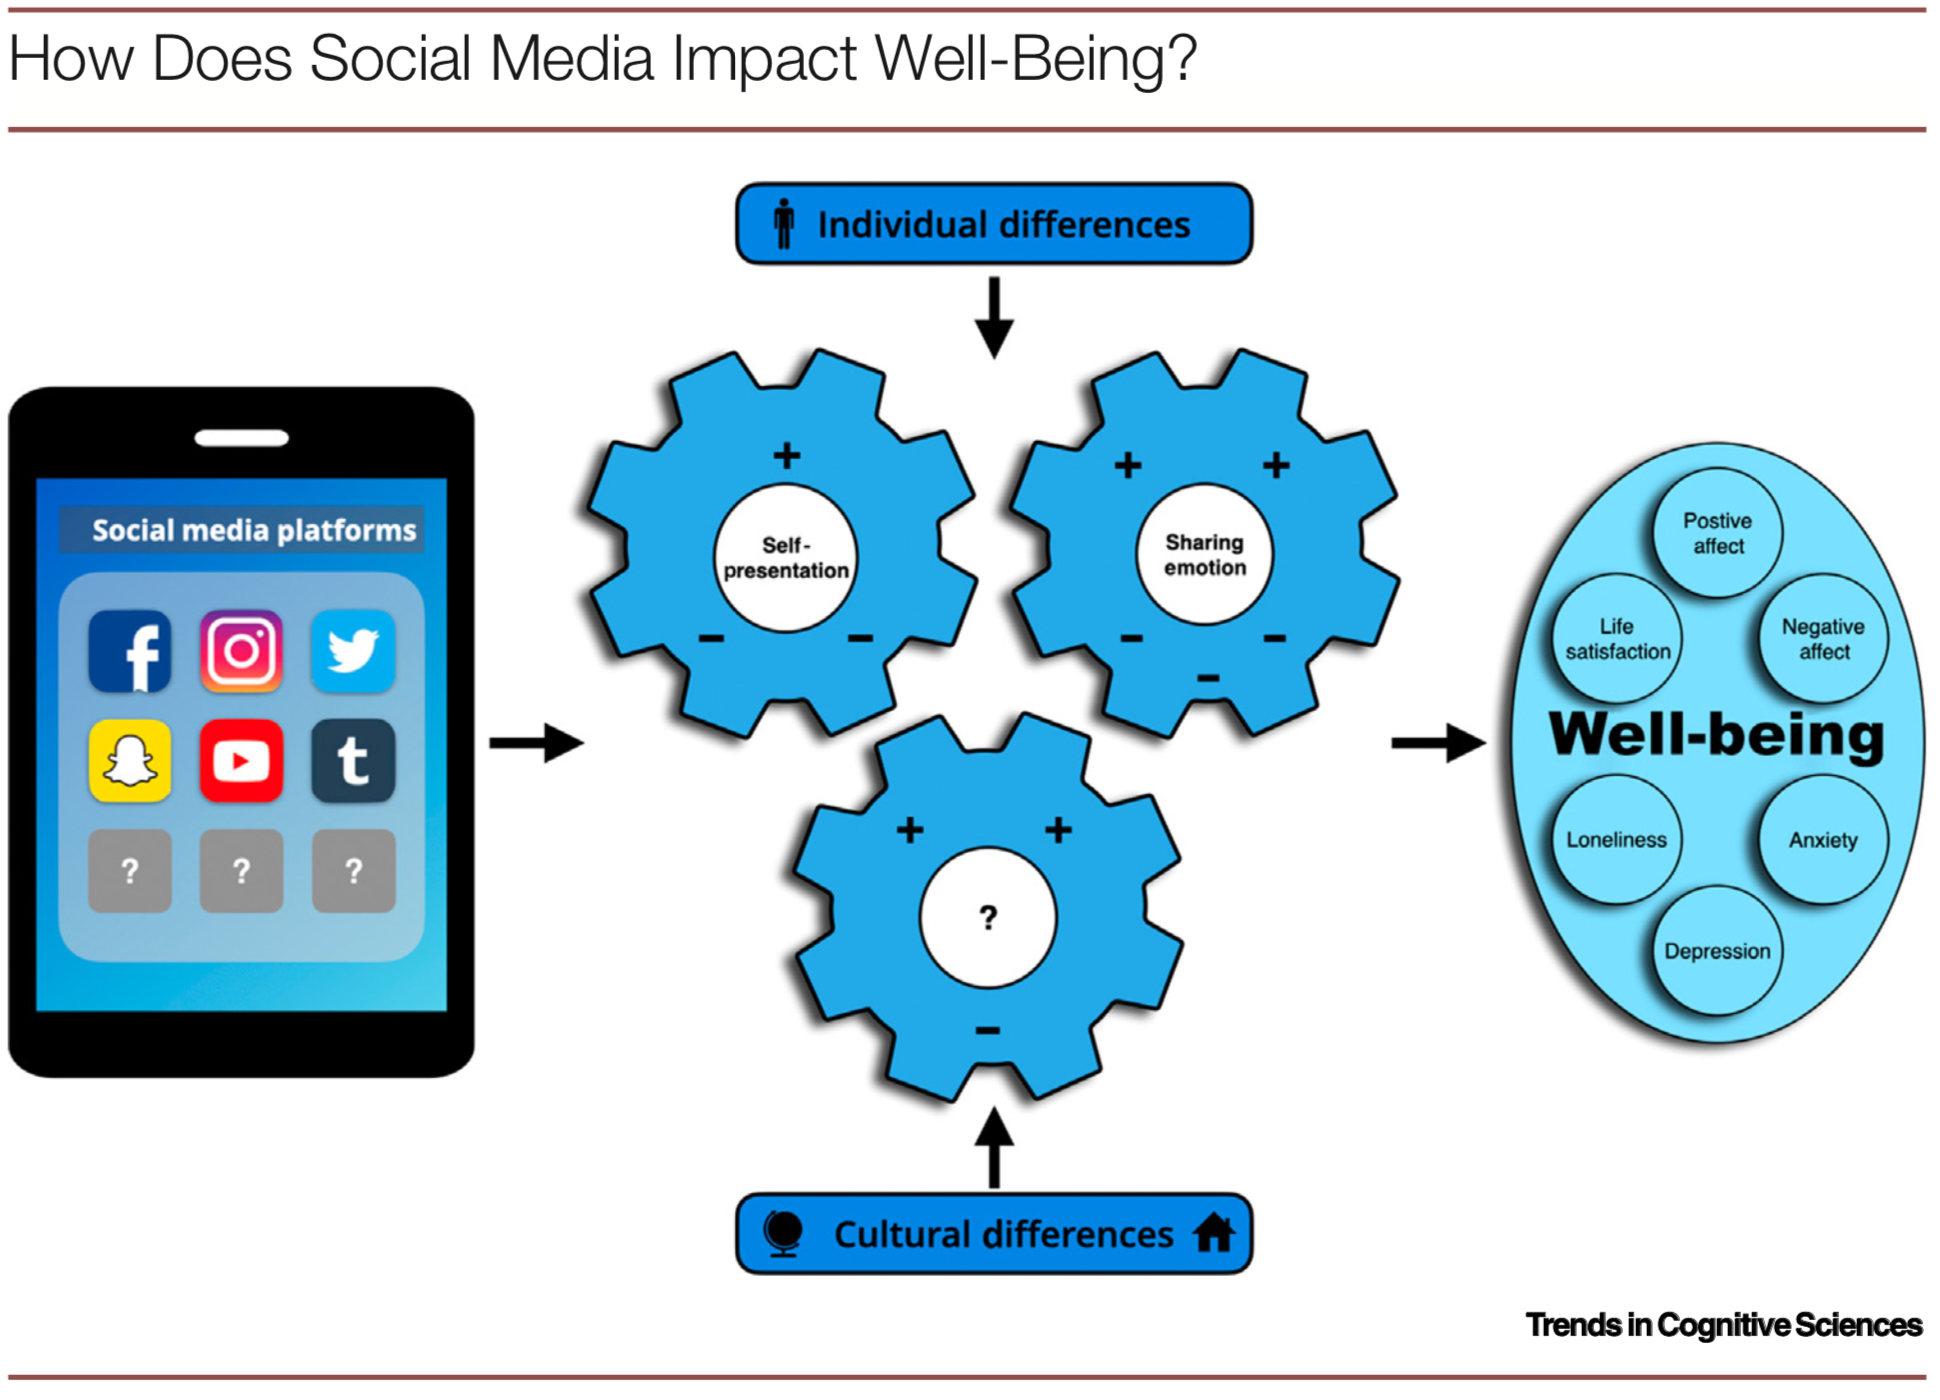
\includegraphics[width=0.8\textwidth]{figures/kross_social_2021_fig1}
\end{center}

\note{
This figure seems like a nice summary.  Many different social media platforms, lots of individual and cultural difference, lots of different outcomes.  this is a recipe for conflicting results
}

\end{frame}
%%%%%%%%%%%%%%%%%%%%%%
\begin{frame}

From what to how
\begin{center}
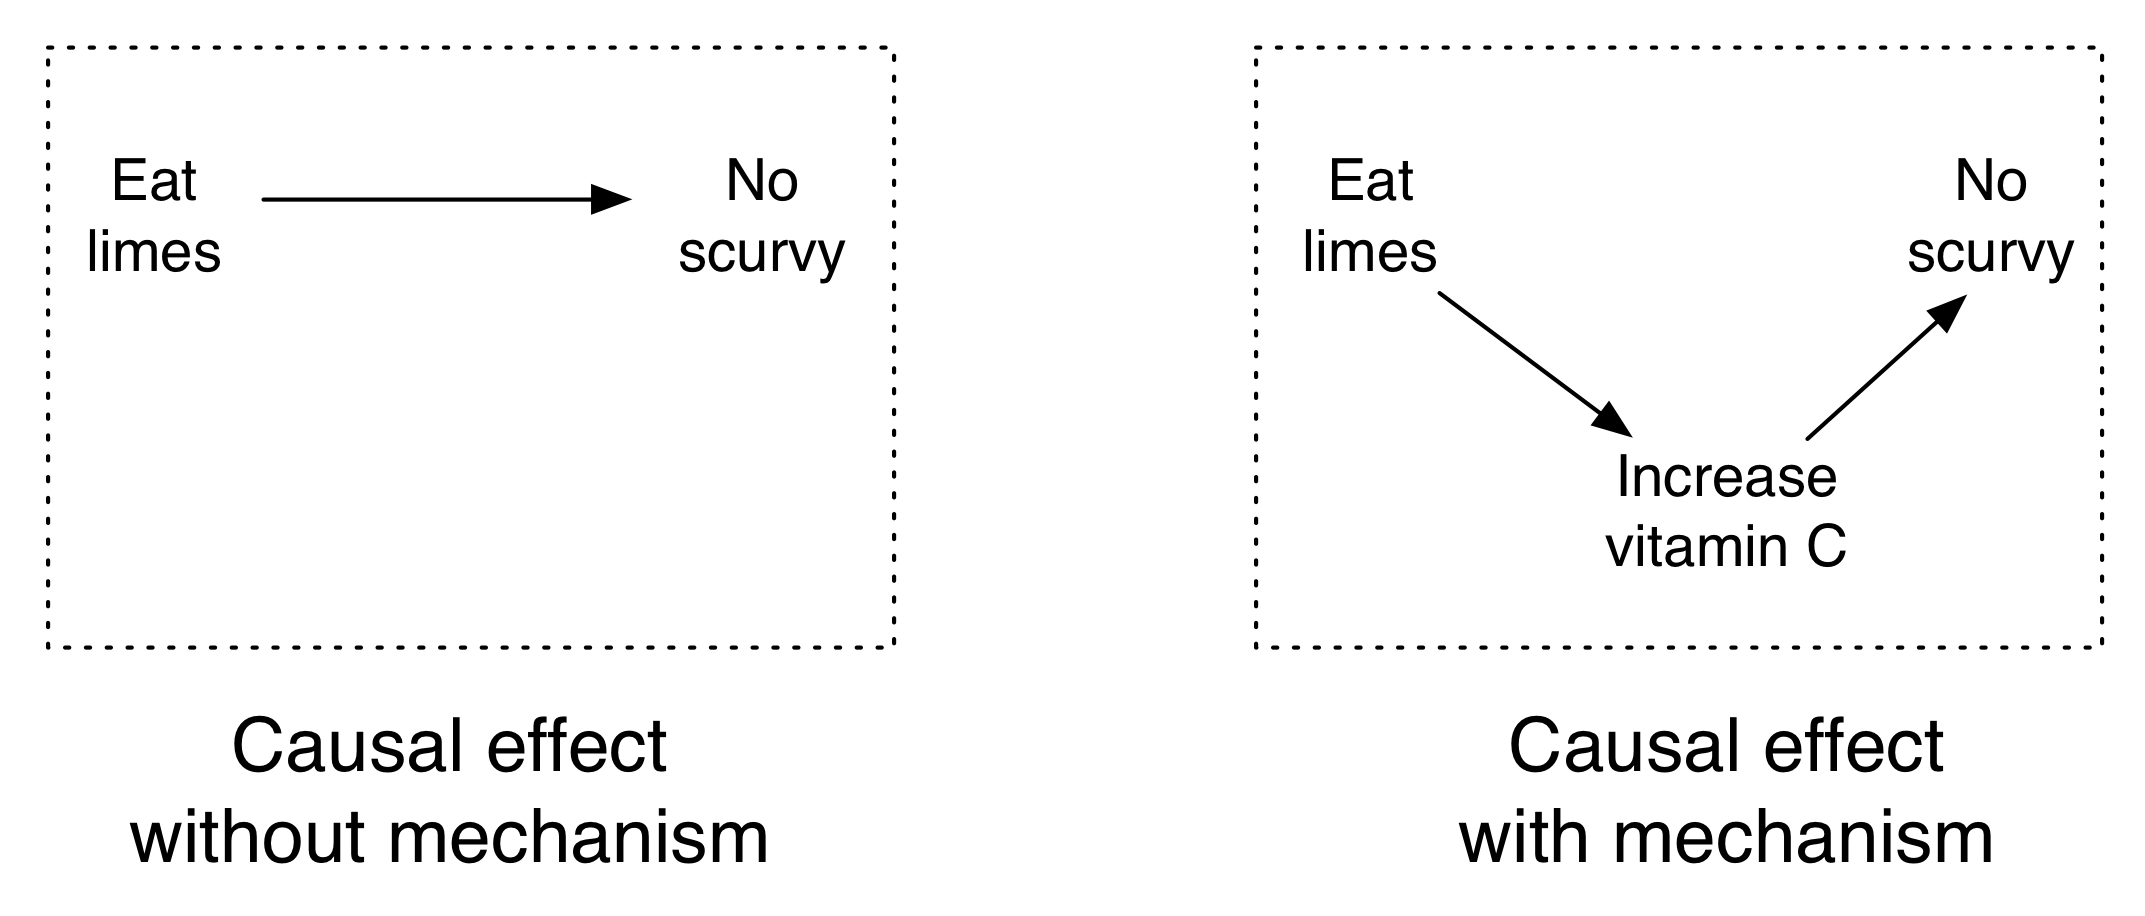
\includegraphics[width=0.8\textwidth]{figures/bitbybit4-10_mechanism_schematic}
\end{center}

\begin{itemize}
\item As you will see in Allcott et al.\ the what questions are easier than the how questions \pause
\item You should think about this as you design your own self-experiment
\end{itemize}

\end{frame}
%%%%%%%%%%%%%%%%%%%%%%
\begin{frame}

What is the effect of Facebook on its users?

\end{frame}


\end{document}
